\documentclass[a4paper]{article}

%--------------------------------------------------------------------------
\usepackage[a4paper, total={6in, 9in}]{geometry}
\usepackage{amsmath}
\usepackage{booktabs}
\usepackage{caption}
\usepackage{graphicx}
\usepackage{float}
\usepackage{inconsolata}
\usepackage{listings}
\usepackage{xcolor}
\usepackage{siunitx}
\usepackage[most]{tcolorbox}
\usepackage{etoolbox}

\makeatletter
\patchcmd{\l@section}
{\hfil}
{\leaders\hbox{\normalfont$\m@th\mkern \@dotsep mu\hbox{.}\mkern \@dotsep mu$}\hfill}
{}{}
\makeatother

%--------------------------------------------------------------------------
\graphicspath{{./fig/}}

%--------------------------------------------------------------------------


\definecolor{mGreen}{rgb}{0,0.6,0}
\definecolor{mGray}{rgb}{0.5,0.5,0.5}
\definecolor{mPurple}{rgb}{0.58,0,0.82}
\definecolor{backgroundColour}{rgb}{0.95,0.95,0.92}

\lstdefinestyle{CStyle}{
	backgroundcolor=\color{backgroundColour},   
	commentstyle=\color{mGreen},
	keywordstyle=\color{magenta},
	numberstyle=\tiny\color{mGray},
	stringstyle=\color{mPurple},
	basicstyle=\footnotesize,
	breakatwhitespace=false,         
	breaklines=true,                 
	captionpos=b,                    
	keepspaces=true,                 
	numbers=left,                    
	numbersep=5pt,                  
	showspaces=false,                
	showstringspaces=false,
	showtabs=false,                  
	tabsize=2,
	language=C
}

\setlength\parindent{0pt}

%--------------------------------------------------------------------------
\begin{document}
\title{HIT332: Embedded and Mobile Systems\\ Practical 5 Notes}
\author{Shane Reynolds}
\maketitle

\tableofcontents

%--------------------------------------------------------------------------
\section{Introduction \& Background}
The intention behind this brief set of notes is to provide guidance on how well the practicals and projects for HIT332: Embedded and Mobile Systems achieve their intended outcomes. There are 5 practicals in total, and 3 projects. This set of notes will cover Practical 5. The practicals (and projects) make use of a development board created by Damien Hill and Ben Saunders of Charles Darwin University. The main component of the board is the Atmel ATmega1281 16au 16MHz, 8-bit microcontroller. The development board can be seen in Figure 1.

\begin{figure}[h]
	\centering
	\frame{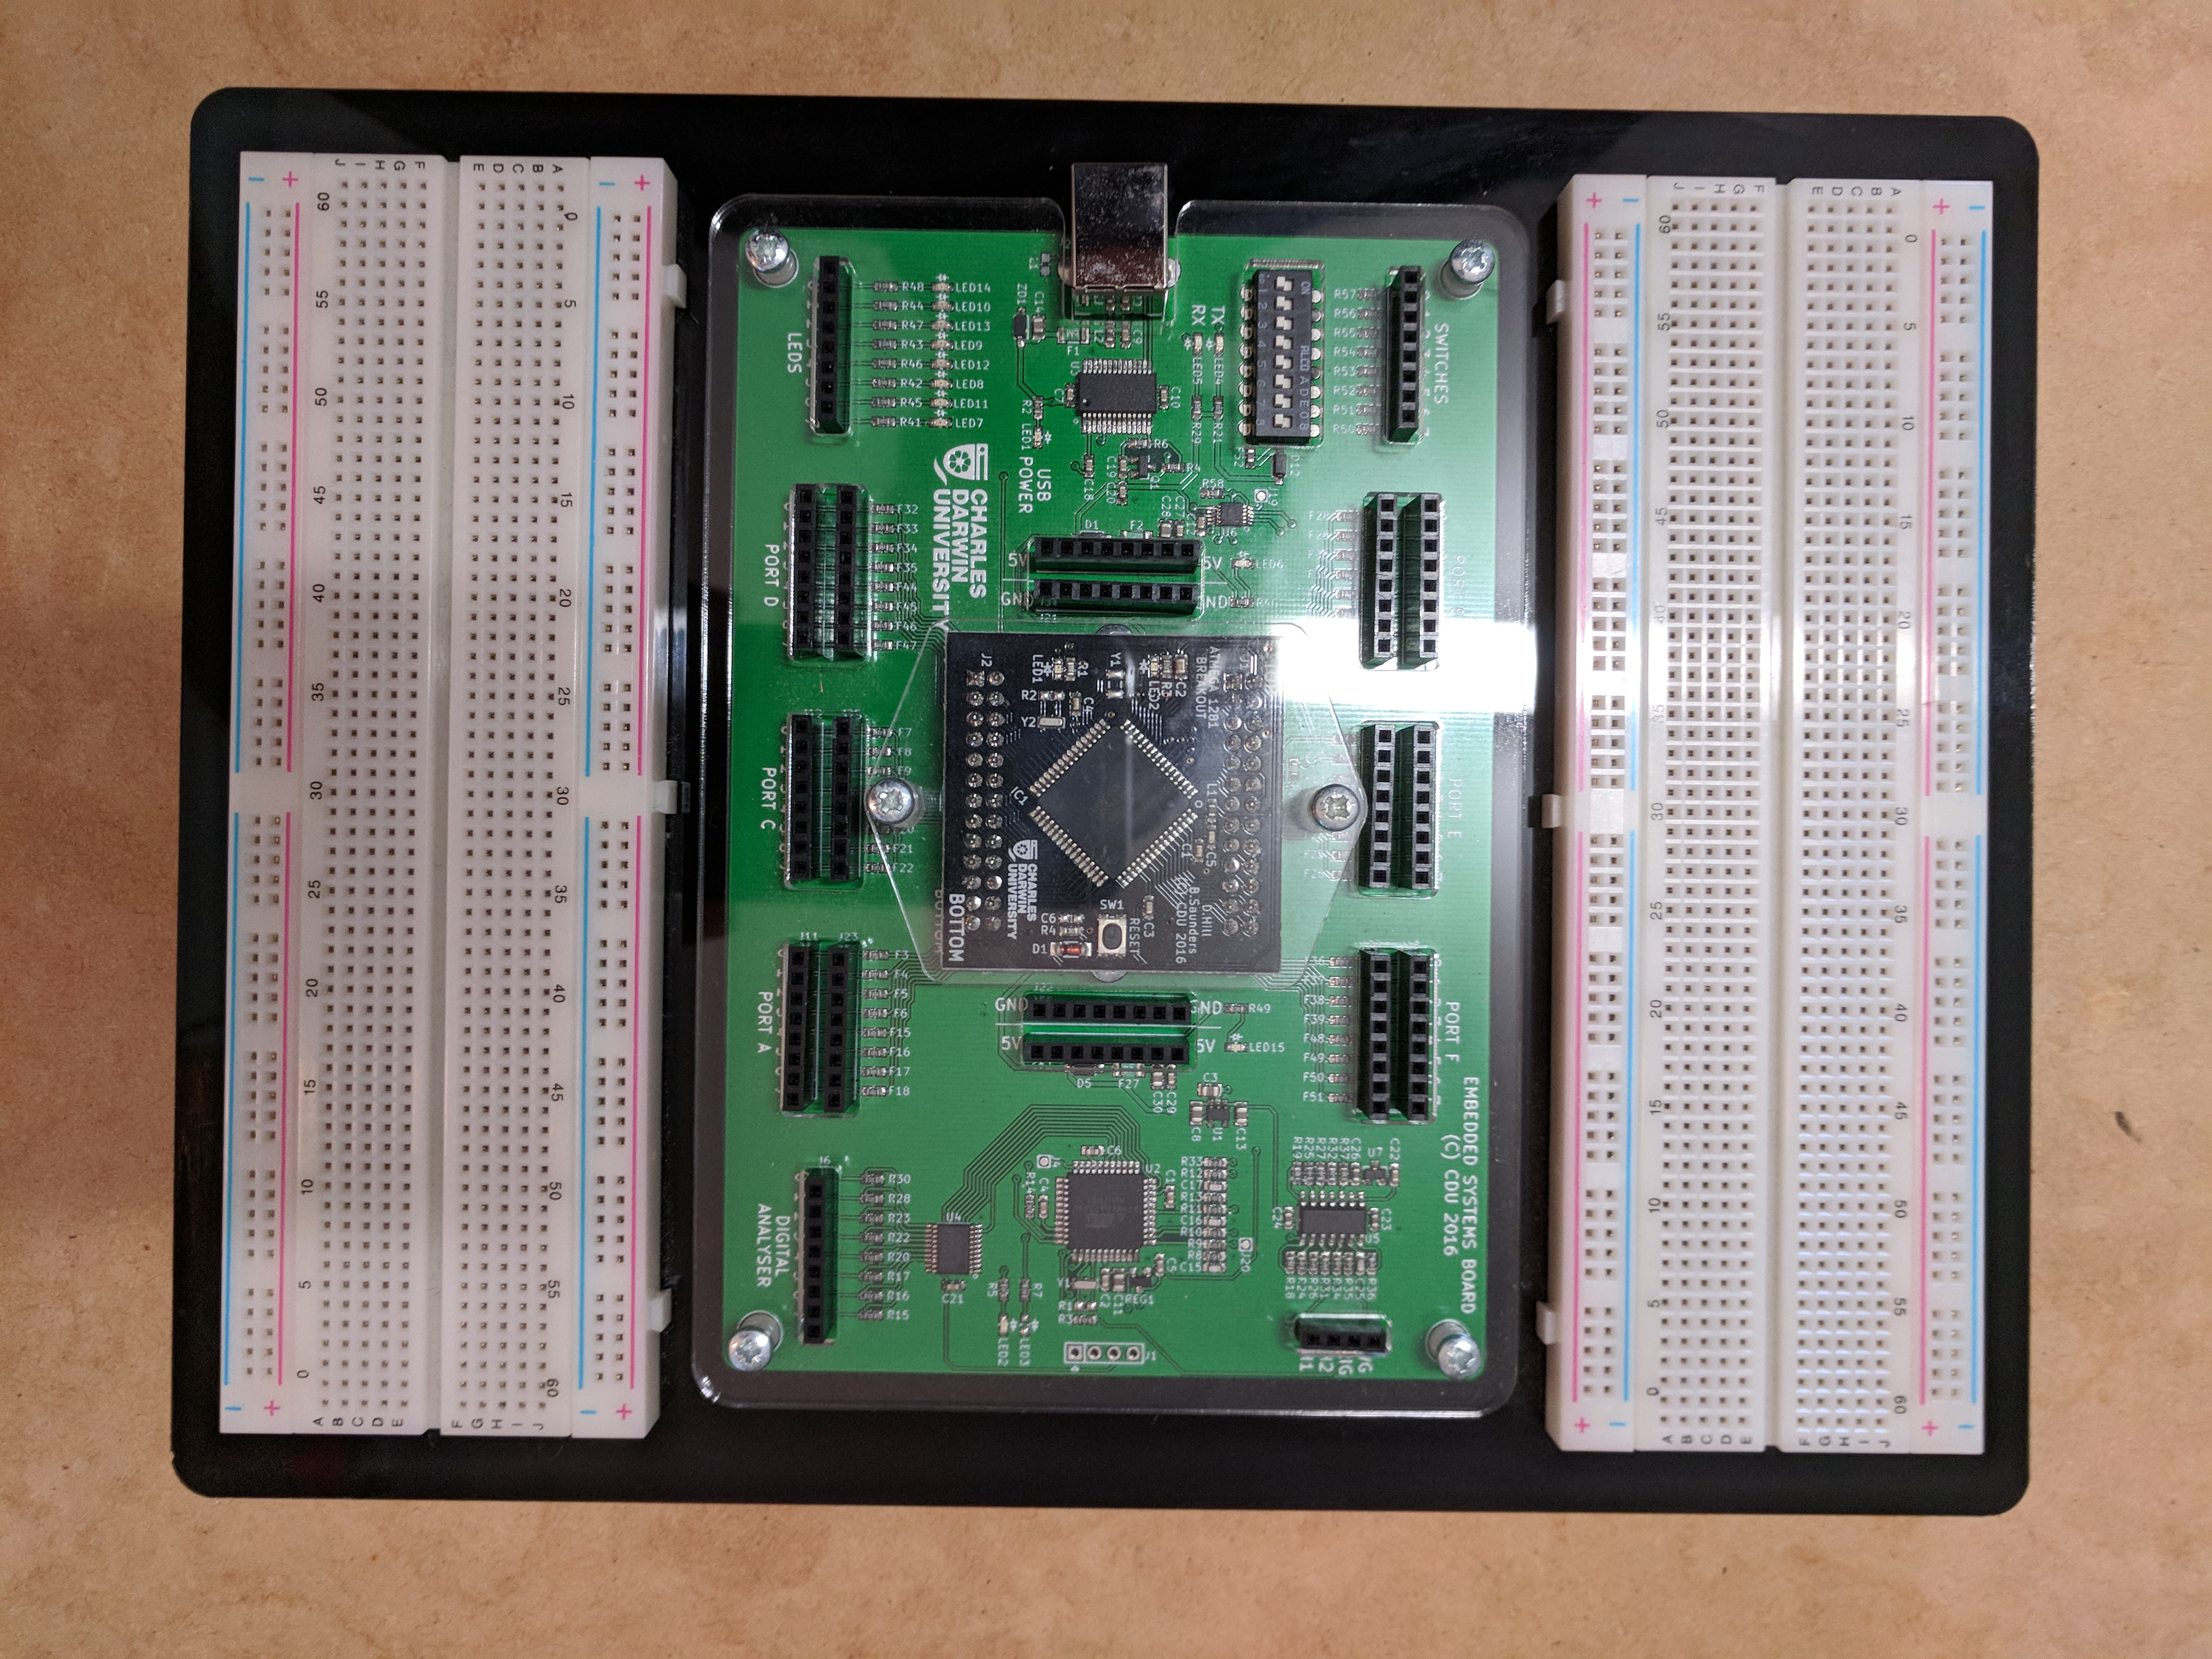
\includegraphics[scale=0.05]{fig1}}
	\caption{The development board which is used in practicals and projects for HIT332: Embedded and Mobile Systems}
\end{figure}

It must be highlighted that these notes have been developed using the board outside of its intended ecosystem. The board is made to be used on CDU's Casuarina Campus in one of the Engineering computer labs. These labs have the appropriate software installed in the correct file paths. These notes have been written using software installed on a personal machine which CDU does not control. Furthermore, the components (other than the development board) used to complete the exercises were sourced independently from a local electronics supplier, independently of CDU. The notes will be highlighted where there has been a significant departure from the intended experience.

\section{USART: Printing to a Terminal}
This section of the practical makes use of basic asynchronous communication with the ATmega1281 - a character will be printed to a terminal window. The USART library was implemented according to the instructions provided in the practical - this simply involved copying the code included in the practical for both the \verb|serial.h| and \verb|serial.c| files. The \verb|main.c| code which was written to print characters to the terminal can be seen in Figure 2 - this was also provided by the practical.

\begin{figure}[h]
	\begin{lstlisting}[style=CStyle]
	#include <avr/io.h>
	#include "serial.h"
	
	int main(void){
	
		unsigned char serialData;
	
		USART_init();
	
		while(1){
			serialData = USART_receive();
			USART_transmit(serialData);
		}
	}
	\end{lstlisting}
	\caption{text}
\end{figure}

The code was programmed into the microcontroller in a similarl fashion to Practical 3, using a modified makefile. To test the code functionality, the Serial Terminal was launched from the CDU Embedded Toolbox, which launched as expected. The Serial terminal performed as intended, and the output can be seen in Figure 3.
\vspace{0.5cm}
\begin{figure}[h]
	\centering
	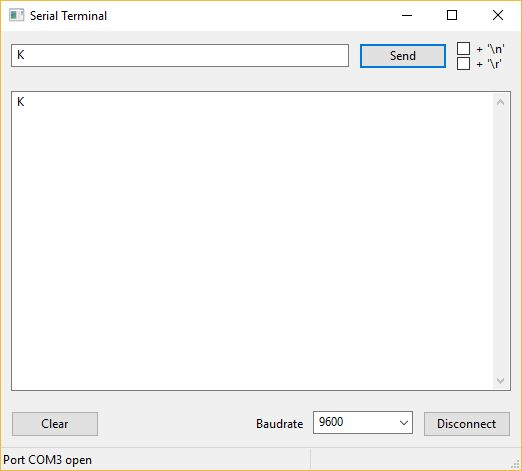
\includegraphics[scale=0.6]{fig2}
	\caption{text}
\end{figure}

\newpage

\section{Analogue to Digital Conversion}
This section of the practical makes use of an analogue to digital (ADC) peripheral included with the microcontroller. A simple analogue temperature sensor (MCP9700) is used to take periodic readings of the ambient temperature, which are sent to a local machine using the serial library, \verb|serial.h| and \verb|serial.c|, developed in Section 1. 
\vspace{1cm}
\begin{figure}[h]
	\centering
	\frame{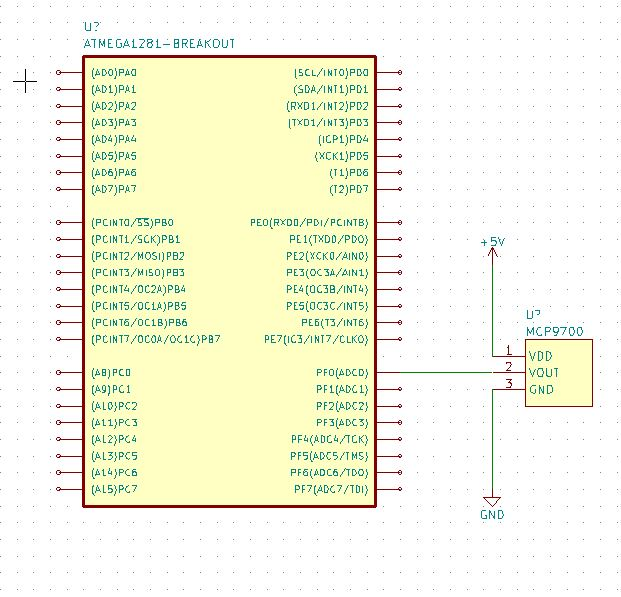
\includegraphics[scale=0.63]{fig3}}
	\caption{text}
\end{figure}
\vspace{1cm}
\begin{figure}[h]
	\centering
	\frame{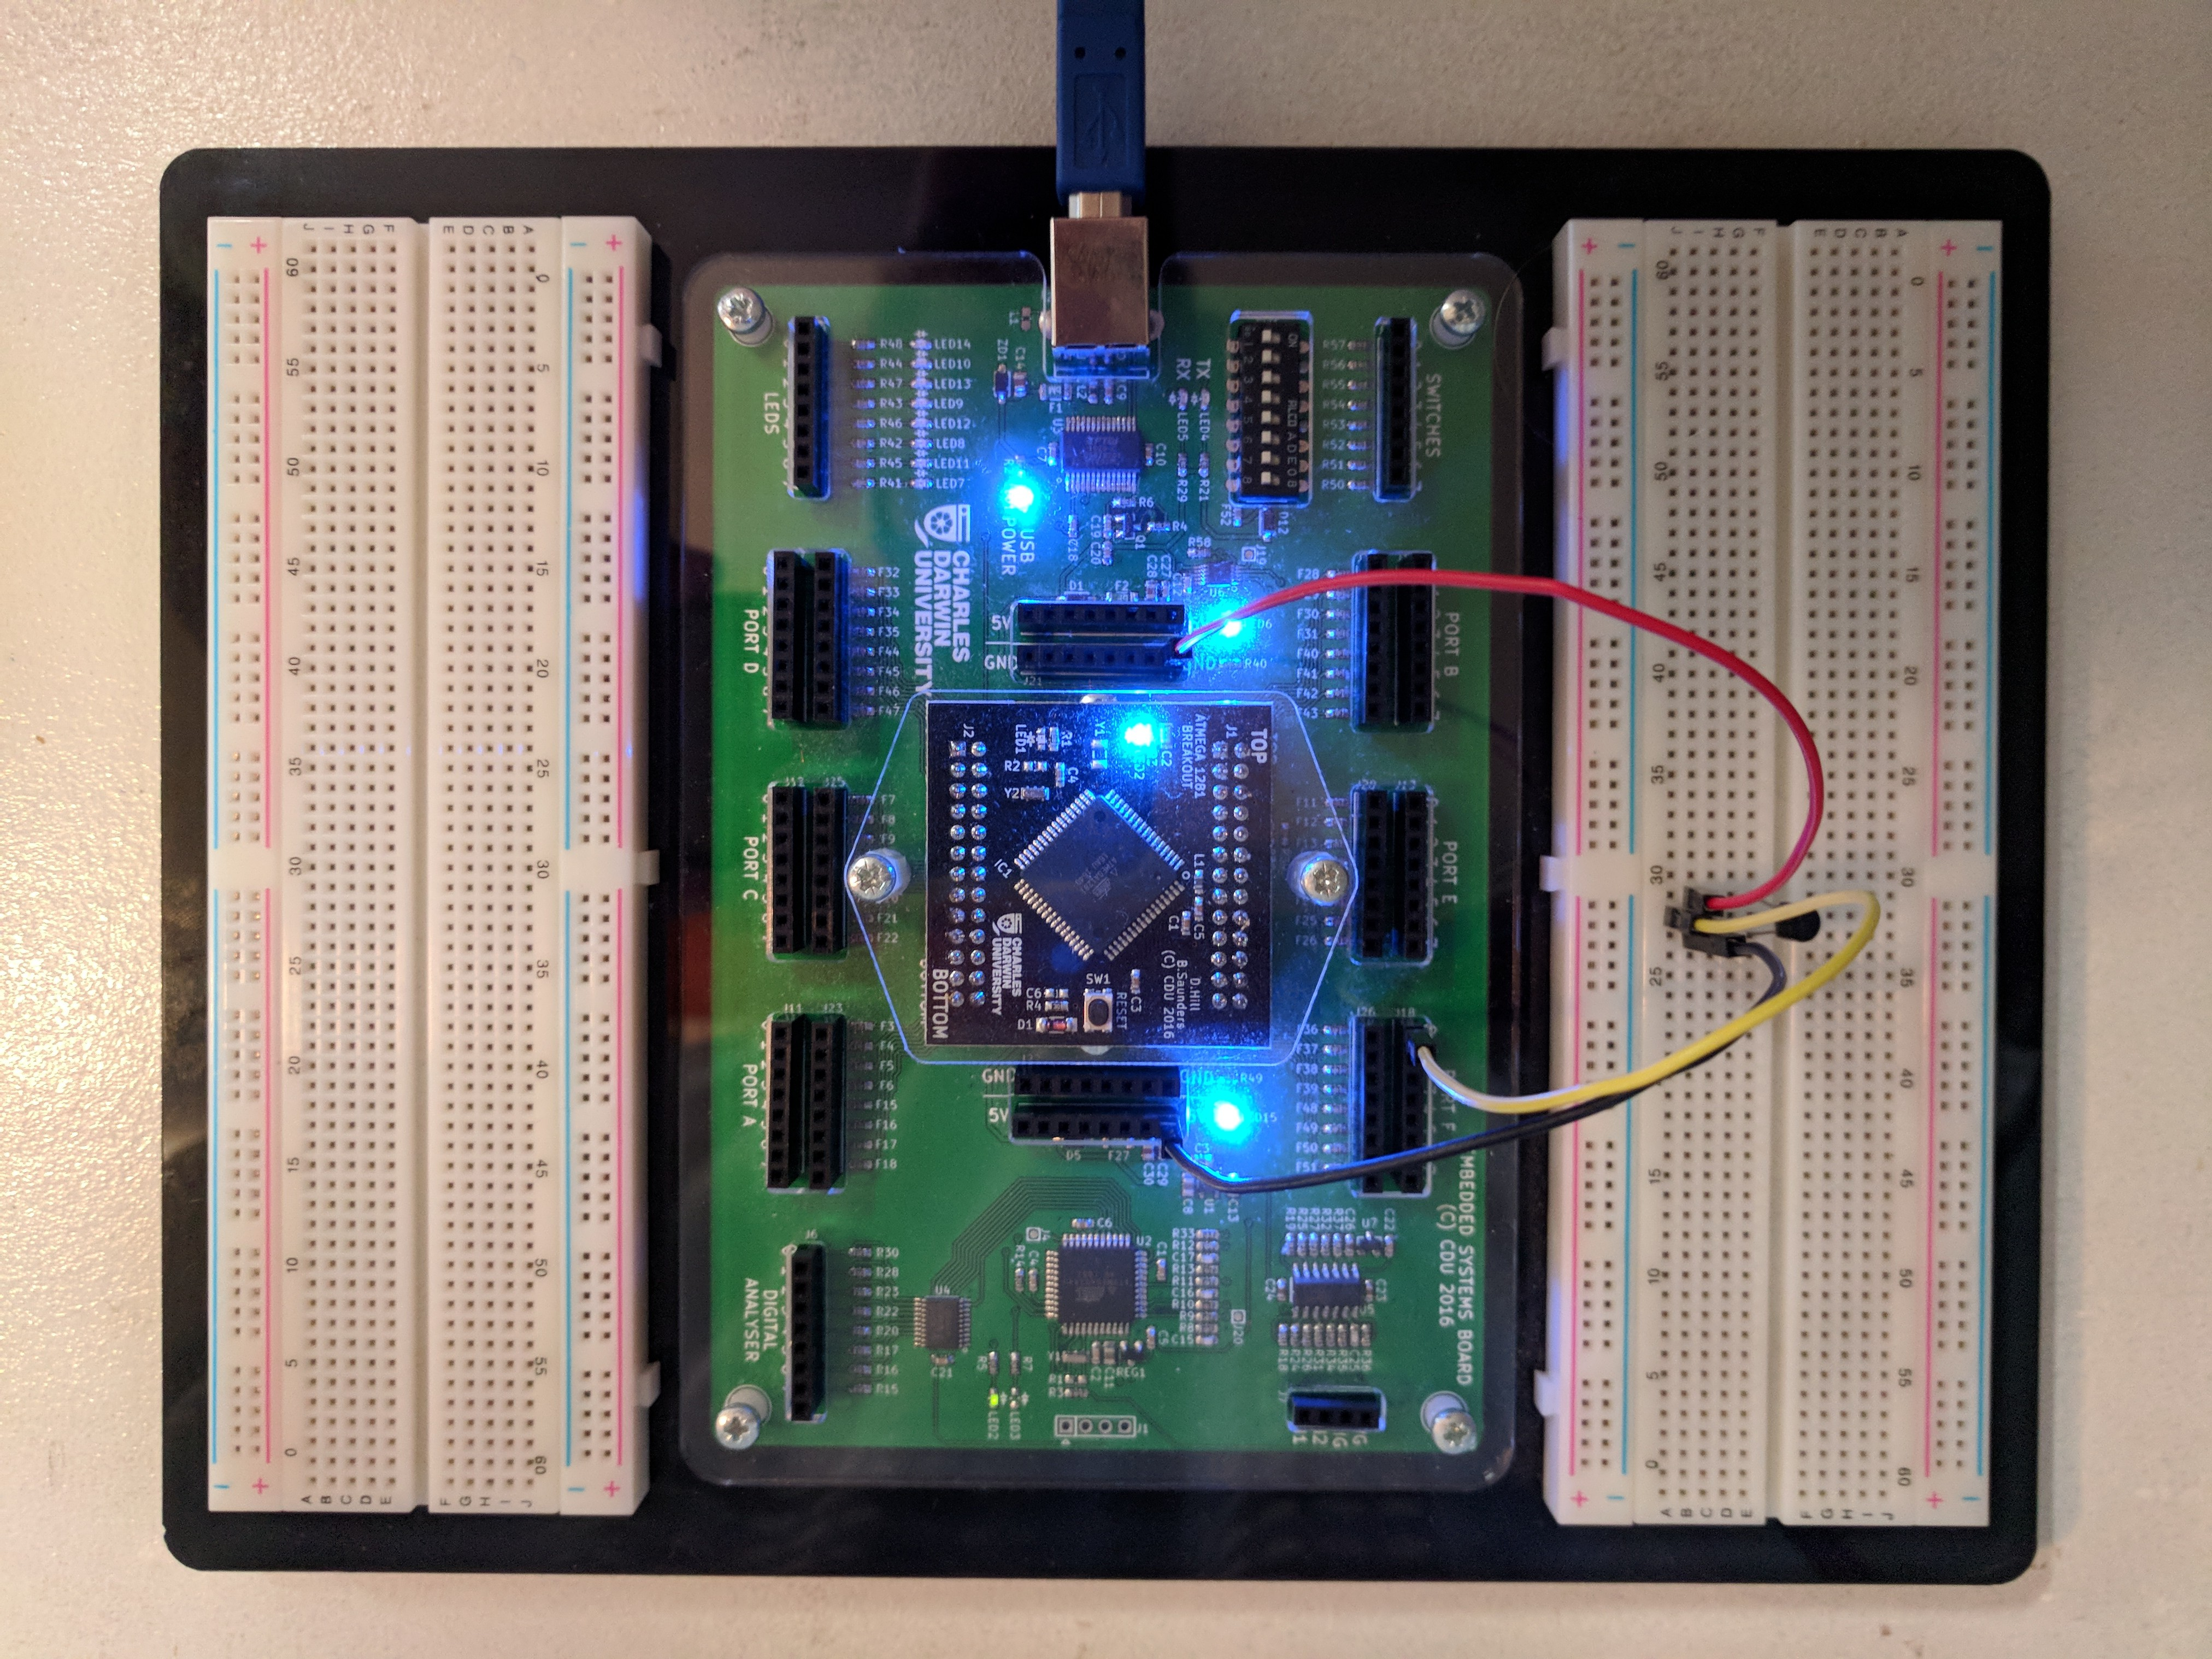
\includegraphics[scale=0.05]{fig5}}
	\caption{text}
\end{figure}

\newpage

It must be noted that the MPC9700 device used for this practical was not provided by CDU, but instead sourced from a local electronics supplier - the device worked as intended. The practical provides detailed instructions to set up the ADC library. This includes copying the code in the instruction and creating the two files \verb|adc.h| and \verb|adc.c| - this library works as intended.\\

The KiCAD schematic of the set up using the MCP9700 can be seen in Figure 4, on the previous page. The physical implementation can be seen in Figure 5, also on the previous page. The \verb|main.c| file which was developed to take ambient temperatures can be seen in Figure 6 - it must be noted that the \verb|serial.h| header file must be included in addition to the \verb|adc.h| header file. The output to the serial terminal can be seen in Figure 7. The practical worked as expected, and the instructions provided were simple to follow, but note that it is important that the student understands, and correctly interprets, the data sheet for the MPC9700.\\
\vspace{1cm}
\begin{figure}[h]
	\begin{lstlisting}[style=CStyle]
	#include <avr/io.h>
	#include <util/delay.h>
	
	#include "serial.h"
	#include "adc.h"
	
	void serial_writeNumber(unsigned int);
	
	int main(void){
		USART_init();
		ADC_init();
	
		while(1){
			unsigned int ADC_value;
			ADC_value = ADC_read(0);
			serial_writeNumber(ADC_value);
			USART_transmit('\n');
			_delay_ms(500);
		}
	}
	
	// Simple function to send a 4 digit positive number as ASCII
	// characters (0-9) over the serial connection.
	// Note that ASCII '0' has a value of 48.
	void serial_writeNumber(unsigned int value){
		unsigned char i;
		if ((value >= 0) && (value <= 9999)){
			i = value/1000;
			USART_transmit(i+48);
			i = (value%1000)/100;
			USART_transmit(i+48);
			i = (value%100)/10;
			USART_transmit(i+48);
			i = (value%10);
			USART_transmit(i+48);
		}
	}
	\end{lstlisting}
	\caption{text}
\end{figure}

\begin{figure}[h]
	\centering
	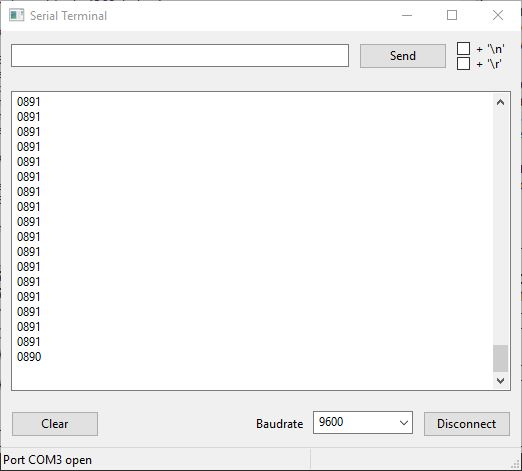
\includegraphics[scale=0.6]{fig6}
	\caption{text}
\end{figure}

\newpage

\section{SPI Communication and Digital Potentiometer}
The final section of this practical has the student use the serial peripheral interface to control a digital potentiometer. The device name is MCP4131. Note that the device used for this practical was not provided by CDU, rather, it was sourced from a local electronics store. The device worked as intended. The practical provides detailed instructions for the creation of \verb|spi.h| and \verb|spi.c|, which worked as intended.\\

\begin{tcolorbox}
\textbf{Attention!!}\\

The practical instructions provided details on how to wire the components in KiCAD, however, it must be noted that the CDU Embedded Toolbox (i.e. the imported KiCAD library developed for this practical) \textbf{did not} appear to contain the MCP4131 component. To work around this I located instructions on the internet detailing how to create and add components to existing KiCAD libraries. The KiCAD schematic can be seen in Figure 8, over the page.
\end{tcolorbox}
\vspace{0.5cm}
The C code which drives the device was provided by the practical instructions and implemented as \verb|main.c| shown in Figure 9, over the page. Note that the \verb|spi.h| header file must be included to ensure this works properly. The device was physically implemented according to the guidance provided. This can be seen in Figure 10, on page 7. Note that like the previous section, this requires the student to read and properly interpret the datasheet in order to successfully navigate the design of the KiCAD schematic, and the physical implementation. Once the program was loaded to the microcontroller, the device worked as expected, and the output of the oscilloscope can be seen in Figure 11, on page 7.

\begin{figure}[h]
	\centering
	\frame{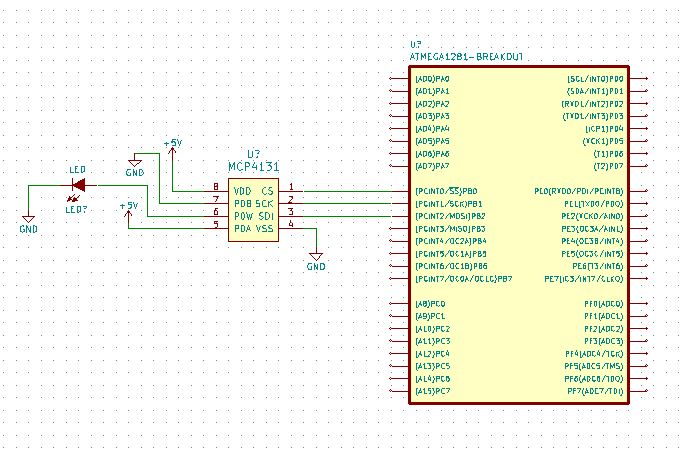
\includegraphics[scale=0.7]{fig9}}
	\caption{text}
\end{figure}

\begin{figure}[h]
	\begin{lstlisting}[style=CStyle]
	#include <avr/io.h>
	#include <util/delay.h>
	
	#include "spi.h"
	
	// function prototypes
	void writeDigitalPot(unsigned char);
	
	int main(void){
		SPI_initMaster();
	
		DDRB |= (1<<PB0);  // set PB0 as output
		PORTB |= (1<<PB0); // set Pb0 highvideo
	
		while(1){
			for (unsigned char i = 0; i<=128; i++){
				writeDigitalPot(i);
				_delay_ms(20);
			}
		}
	}
	
	// function to write a value to the MCP4131
	// digital potentiometer
	void writeDigitalPot(unsigned char value){
		PORTB &= ~(1<<PB0);		// set PB0 low to pull CS low
		SPI_readWrite(0);		// send address byte
		SPI_readWrite(value);	// send potentiometer value
		PORTB |= (1<<PB0);		// set PB0 high
	}
	\end{lstlisting}
	\caption{text}
\end{figure}

\begin{figure}[h]
	\centering
	\frame{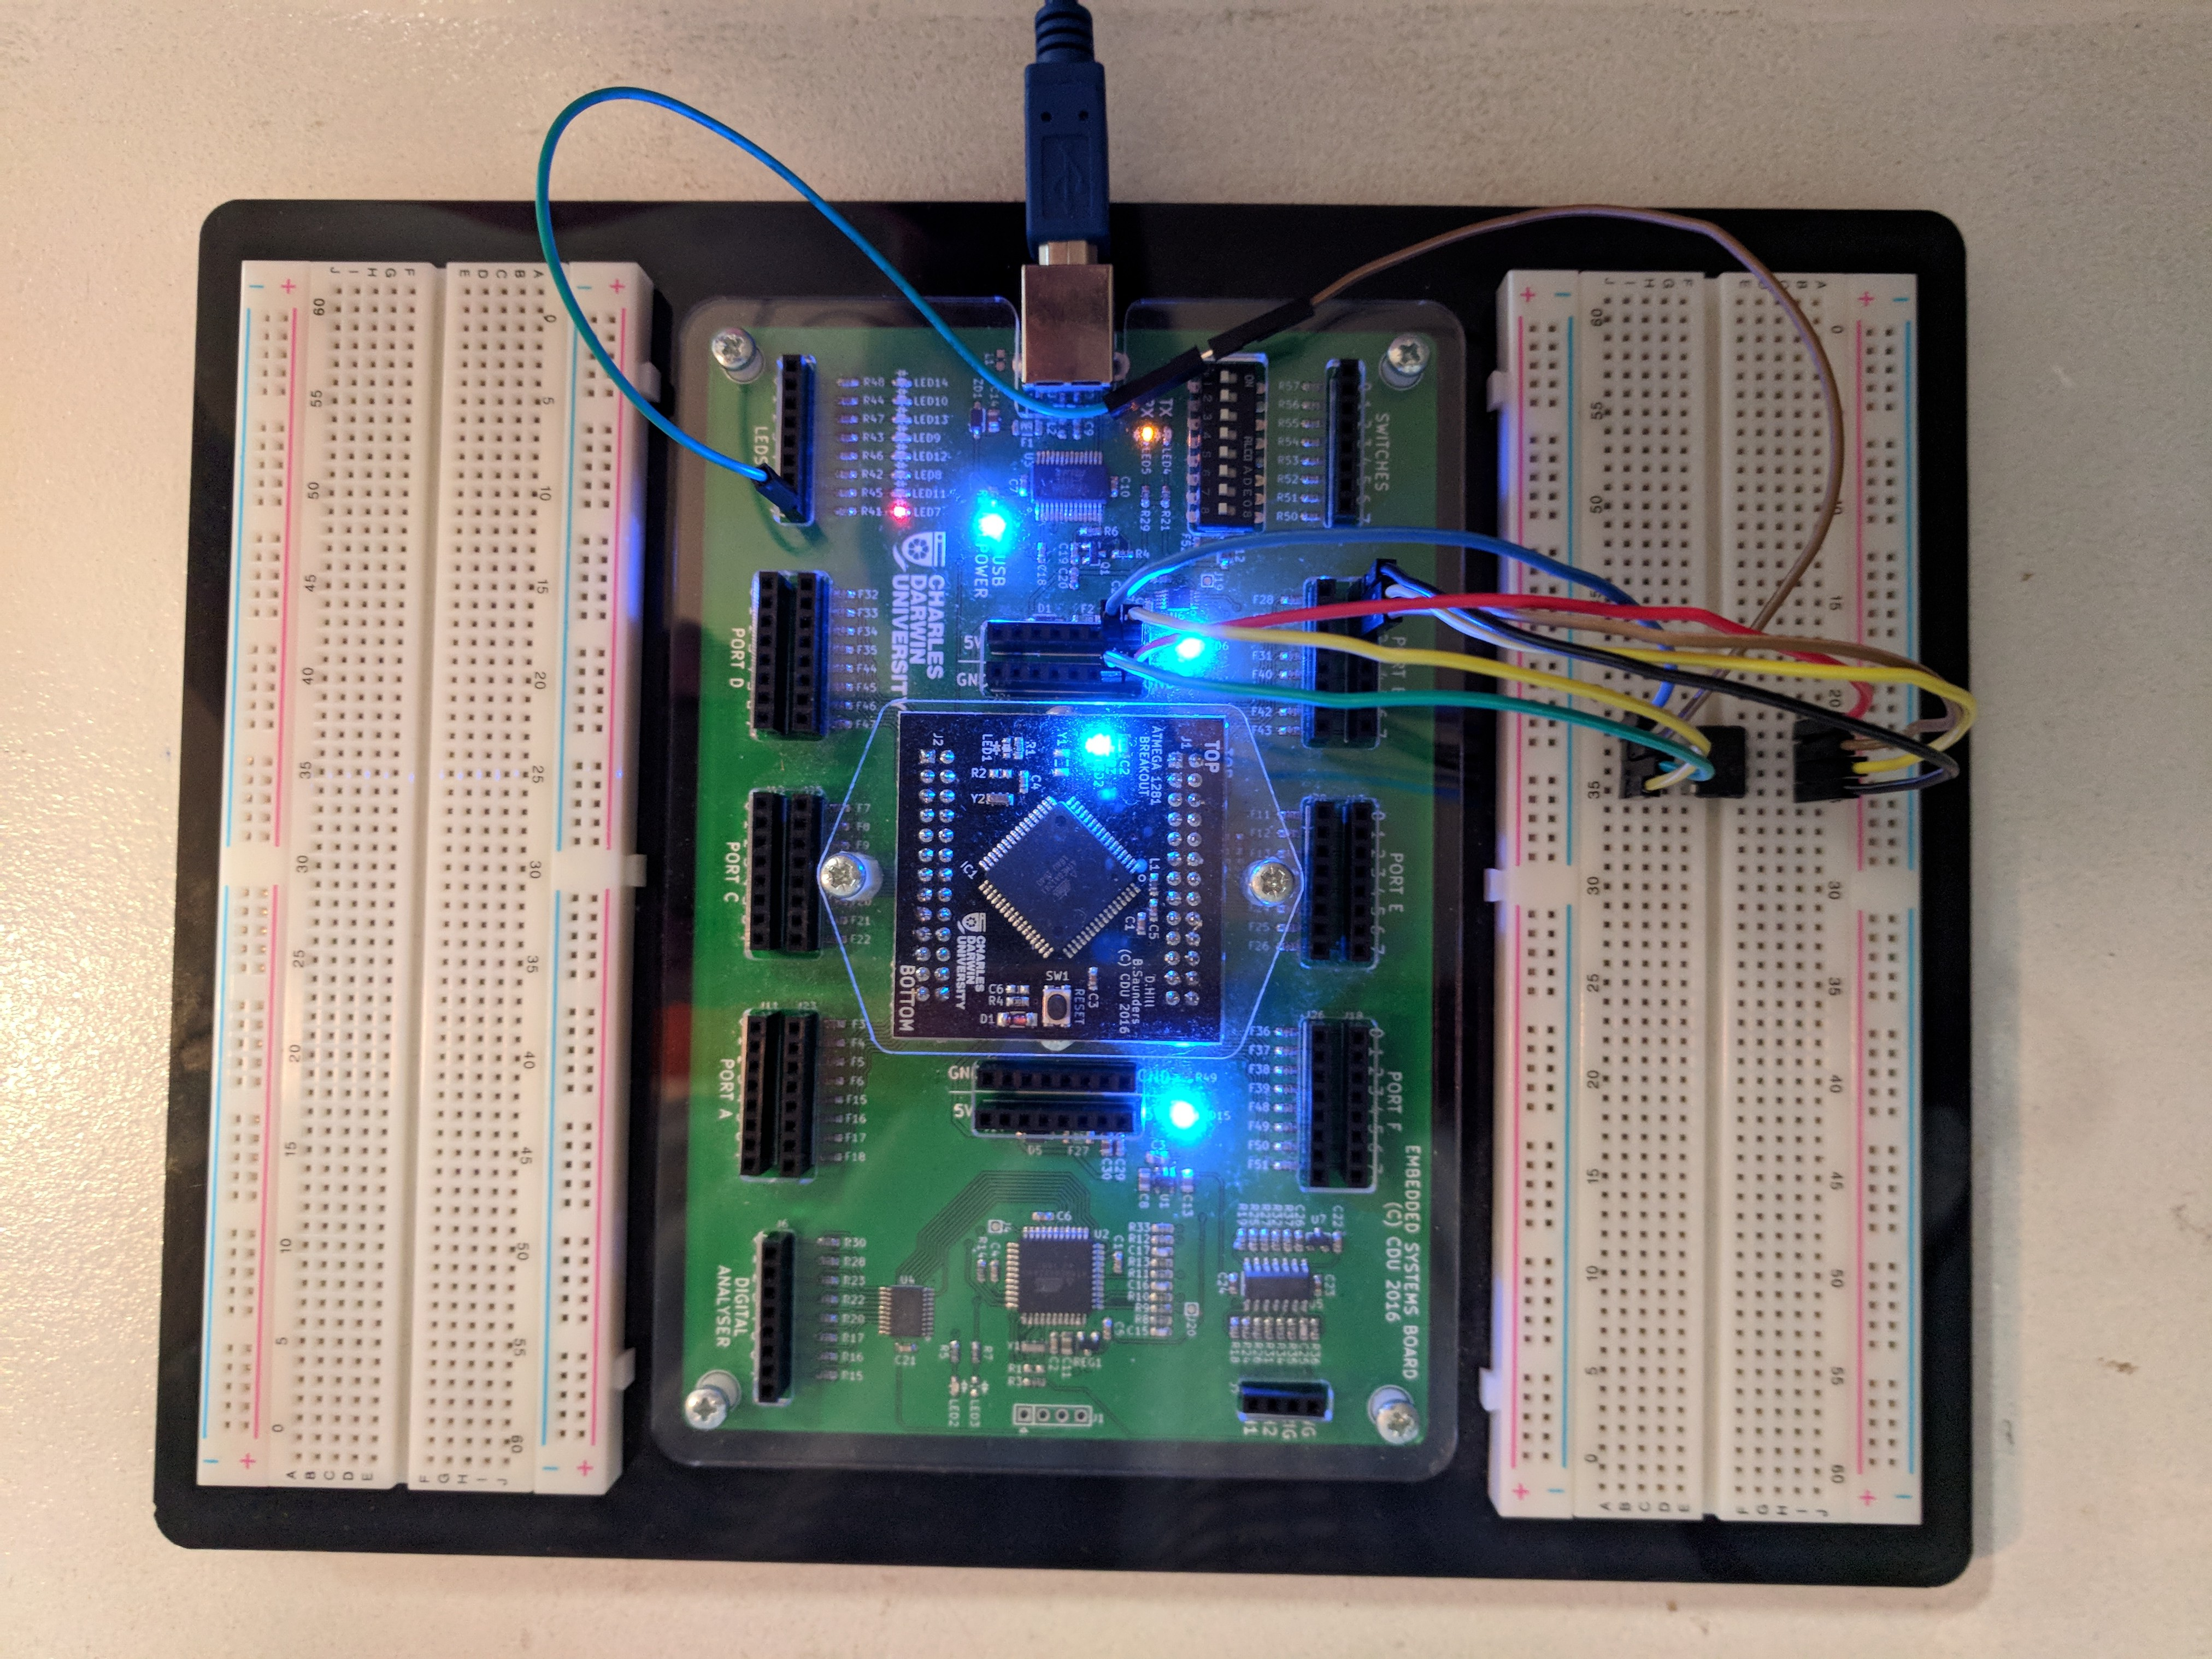
\includegraphics[scale=0.05]{fig7}}
	\caption{text}
\end{figure}

\begin{figure}
	\centering
	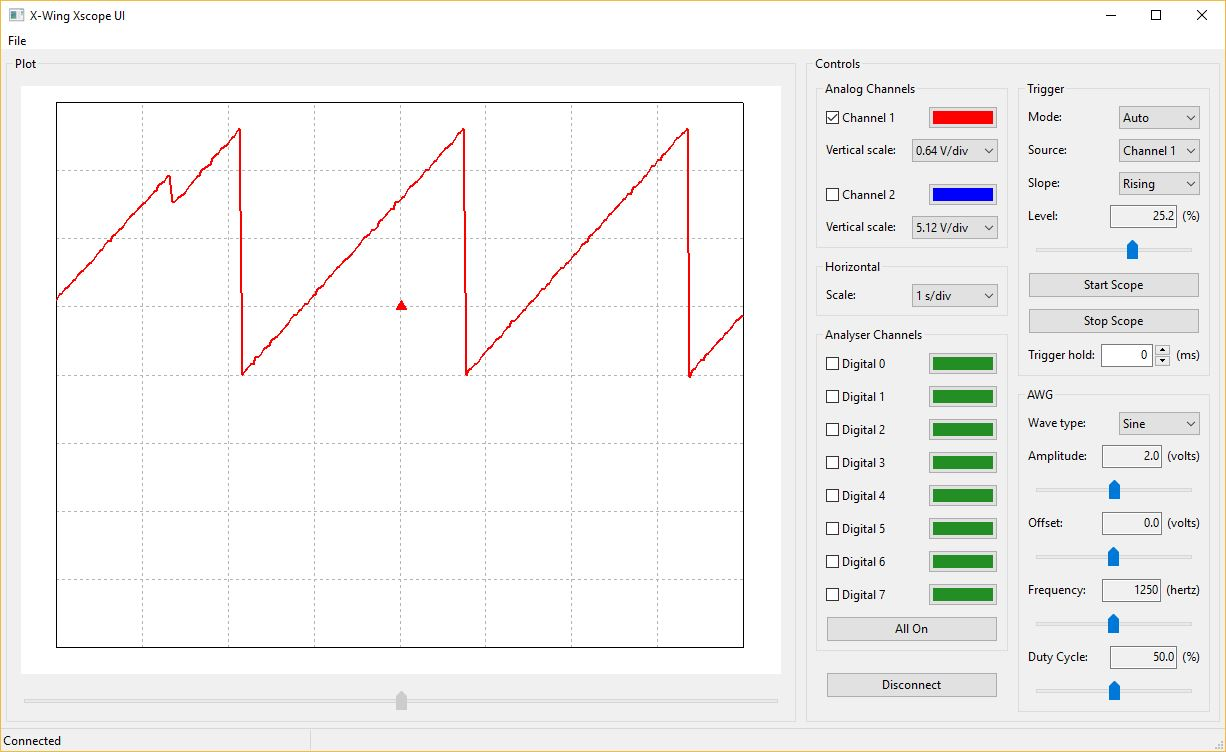
\includegraphics[scale=0.5]{fig8}
	\caption{text}
\end{figure}

\end{document}